\let\negmedspace\undefined
\let\negthickspace\undefined
\documentclass[journal]{IEEEtran}
\usepackage[a5paper, margin=10mm, onecolumn]{geometry}
%\usepackage{lmodern} % Ensure lmodern is loaded for pdflatex
\usepackage{tfrupee} % Include tfrupee package

\setlength{\headheight}{1cm} % Set the height of the header box
\setlength{\headsep}{0mm}     % Set the distance between the header box and the top of the text

\usepackage{gvv-book}
\usepackage{gvv}
\usepackage{cite}
\usepackage{amsmath,amssymb,amsfonts,amsthm}
\usepackage{algorithmic}
\usepackage{graphicx}
\usepackage{textcomp}
\usepackage{xcolor}
\usepackage{txfonts}
\usepackage{listings}
\usepackage{enumitem}
\usepackage{mathtools}
\usepackage{gensymb}
\usepackage{comment}
\usepackage[breaklinks=true]{hyperref}
\usepackage{tkz-euclide} 
\usepackage{listings}
% \usepackage{gvv}                                        
\def\inputGnumericTable{}                                 
\usepackage[latin1]{inputenc}                                
\usepackage{color}                                            
\usepackage{array}                                            
\usepackage{longtable}                                       
\usepackage{calc}                                             
\usepackage{multirow}                                         
\usepackage{hhline}                                           
\usepackage{ifthen}
\usepackage{lscape}
\begin{document}

\bibliographystyle{IEEEtran}



\title{4.3.47}
\author{EE25BTECH11057 - Rushil Shanmukha Srinivas
}
% \maketitle
% \newpage
% \bigskip
{\let\newpage\relax\maketitle}

\renewcommand{\thefigure}{\theenumi}
\renewcommand{\thetable}{\theenumi}
\setlength{\intextsep}{10pt} % Space between text and floats

\numberwithin{equation}{enumi}
\numberwithin{figure}{enumi}
\renewcommand{\thetable}{\theenumi}

\textbf{Problem:} Find the equation of the line through (-2,3) with slope -4.

\textbf{Solution:}
Given point is 
\begin{align}
\vec{h}=\myvec
{-2\\3} , Slope=m=-4
\end{align}
The equation of the line is given by
\begin{align}
y=mx+c
\end{align}
\begin{align}
\myvec{x\\y} = \myvec{x\\mx+c}=\myvec{0\\c} + x\myvec{1\\m}
\end{align}
So
\begin{align}
\vec{n}^\top \vec{x} = \vec{n}^\top \vec{h} =c
\end{align}
 where $\vec{h}$ is any point on the line and $\vec{n}=\myvec{-m\\1} $
\begin{align}
c = \vec{n}^\top \vec{h} = \myvec{4 & 1}\myvec{-2\\3} = -5
\end{align}
so equation of line is 
\begin{align}
y=-4x -5 
\end{align}
 
\begin{figure}[h!]
  \centering
  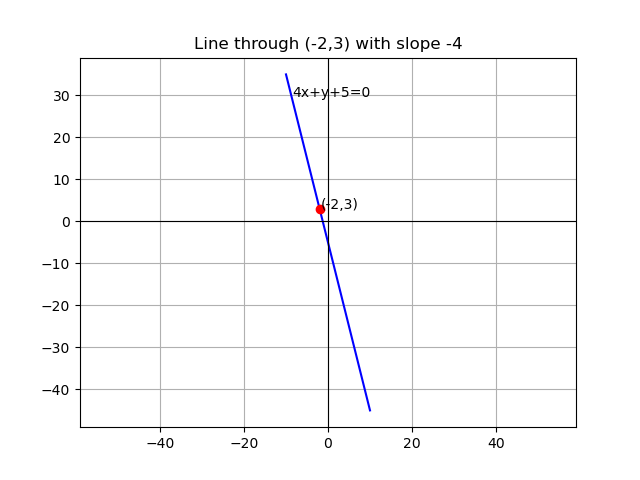
\includegraphics[width=0.9\columnwidth]{figs/fig6.png} 
   \caption*{Fig: Representation of Line and Point}
  \label{Fig6}
\end{figure}

\end{document}


